\documentclass[conference]{IEEEtran}
\IEEEoverridecommandlockouts
\usepackage{cite}
\usepackage{amsmath,amssymb,amsfonts}
\usepackage{graphicx}
\usepackage{textcomp}
\usepackage{xcolor}
\usepackage{booktabs}
\usepackage{multirow}
\usepackage{tikz}
\usetikzlibrary{positioning,arrows.meta}

\begin{document}

\title{Acoustic Forensics: A Stacked Ensemble of CRNN and Classical Models for Synthetic Speech Detection}

\author{
\IEEEauthorblockN{VeriVox Research Team}
\IEEEauthorblockA{\textit{Department of Information Technology} \\
\textit{Indian Institute of Information Technology, Allahabad}\\
Prayagraj, Uttar Pradesh, India \\
forensics@iiita.ac.in}
}

\maketitle

\begin{abstract}
Synthetic speech generated by advanced deep neural text-to-speech (TTS) and voice conversion (VC) architectures poses severe risks to biometric speaker verification, legal evidence authenticity, and digital communication integrity. We present \textit{Acoustic Forensics}, an end-to-end detection pipeline that couples six heterogeneous classifiers through stacked generalization. The ensemble integrates two deep Convolutional Recurrent Neural Networks (CRNN) with multi-head self-attention operating over linear frequency cepstral coefficients (LFCC) and log-mel filterbanks, alongside four classical models: a 64-component Gaussian Mixture Model (GMM), an RBF Support Vector Machine (SVM), a Random Forest, and a Logistic Regression baseline. Base model continuous scores are standardized against validation statistics and fused via an $L_2$-regularized Logistic Regression meta-learner fitted strictly on the development partition to enforce a zero-leakage protocol. The system delivers a calibrated probability of authenticity, an explicit uncertainty band for borderline scores ($P \in [0.40, 0.60]$), and frame-level temporal attention salience maps for forensic interpretability. Evaluated on the complete ASVspoof 2019 Logical Access (LA) evaluation set (71{,}237 trials), our primary CRNN-LFCC achieves an Equal Error Rate (EER) of 6.70\% (min-tDCF 0.2143, ROC-AUC 0.9800), while the stacked ensemble achieves 10.74\% EER (min-tDCF 0.2754), consistently outperforming unweighted baseline score fusion (11.47\% EER, min-tDCF 0.3077). In zero-shot cross-domain testing on the unconstrained In-the-Wild dataset (25{,}589 clips), the detector records an optimal EER of 44.73\% (ROC-AUC 0.5638). Extensive stress-testing under MP3, AAC, and Opus compression (16--64\,kbps) confirms that Opus and AAC preserve countermeasure discriminability substantially better than MP3.
\end{abstract}

\begin{IEEEkeywords}
audio deepfake detection, acoustic forensics, anti-spoofing, ASVspoof 2019, stacked ensemble, CRNN, LFCC, attention salience
\end{IEEEkeywords}

\section{Introduction and Related Work}
Recent breakthroughs in deep generative modeling, including neural vocoders (e.g., WaveNet, WaveRNN, HiFi-GAN) and sequence-to-sequence acoustic synthesizers, enable the synthesis of highly naturalistic synthetic speech and voice clones using only brief reference audio. When deployed maliciously, automated voice spoofing threatens voice-biometric authentication in financial banking, enables targeted social engineering fraud, and undermines the evidentiary value of recorded voice in judicial proceedings \cite{wang2020asvspoof,muller2022does}.

In response, countermeasure research has progressed through competitive evaluations such as the ASVspoof challenge series \cite{wang2020asvspoof,todisco2019asvspoof}. Early countermeasures paired hand-crafted acoustic representations with statistical spectral models. In particular, Linear Frequency Cepstral Coefficients (LFCC) demonstrated decisive advantages over conventional Mel-Frequency Cepstral Coefficients (MFCC) because linear filterbank spacing preserves high-frequency spectral flux and harmonic phase incoherence introduced by vocoder synthesis, whereas psychoacoustic mel-warping excessively compresses spectral detail above 4\,kHz \cite{sahidullah2015comparison}.

Subsequent research shifted toward deep neural architectures processing static 2D spectrogram representations or raw time-domain waveforms. Representative systems include Light Convolutional Neural Networks (LCNN) employing Max-Feature-Map (MFM) activation functions to filter low-magnitude synthetic noise \cite{lavrentyeva2019stc}, raw-waveform models such as RawNet2 utilizing sinc-convolution filters \cite{tak2021rawnet2}, and spectro-temporal graph attention networks such as AASIST \cite{jung2022aasist}. Despite notable benchmark success, existing models suffer from two primary limitations:
\begin{enumerate}
    \item \textbf{Generalization Brittleness:} Deep detectors often overfit to idiosyncratic synthesis artifacts present in training sets, suffering severe performance collapse when confronted with unseen generative techniques or acoustic mismatch \cite{muller2022does}.
    \item \textbf{Forensic Opacity and Calibration Deficits:} Autonomous countermeasures frequently produce uncalibrated logits that lack probabilistic meaning and provide no temporal localization of fraudulent segments, rendering them inadequate for courtroom forensic standards.
\end{enumerate}

To overcome these challenges, we adopt Wolpert's stacked generalization paradigm \cite{wolpert1992stacked}. Rather than relying on a solitary classifier, our architecture harnesses a heterogeneous ensemble comprising deep spatial-recurrent networks alongside statistical frame-level and subspace models. Our core contributions are:
\begin{itemize}
    \item \textbf{Heterogeneous Stacked Ensemble:} A principled six-model detector spanning linear and mel representations, coupled through an $L_2$-regularized meta-learner fitted strictly on validation scores under an airtight zero-data-leakage protocol.
    \item \textbf{Calibrated Forensic Output and Attention Salience:} Production of calibrated posterior probabilities $P(\text{bona fide})$, an uncertainty region for margin decisions ($P \in [0.40, 0.60]$), and multi-head temporal self-attention heatstrips identifying specific spoofed phonemes.
    \item \textbf{Comprehensive Stress-Testing and Zero-Shot Audits:} Detailed empirical evaluations across all 13 unseen ASVspoof 2019 evaluation attacks (A07--A19), lossy telephony/streaming codec chains (MP3, AAC, Opus at 16--64\,kbps), voice activity detection (VAD) silence-shortcut bias tests, and zero-shot cross-domain generalization on the unconstrained In-the-Wild corpus.
\end{itemize}

\section{Methodology}
Fig.~\ref{fig:pipeline} outlines the end-to-end Acoustic Forensics pipeline. Raw audio undergoes signal conditioning, dual-branch spectral extraction, multi-model scoring, validation-anchored score standardization, and stacker fusion.

\begin{figure}[htbp]
\centering
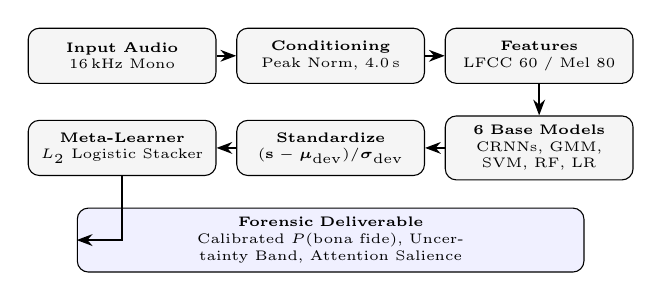
\begin{tikzpicture}[node distance=0.25cm and 0.25cm, every node/.style={font=\tiny}, b/.style={draw,rounded corners,align=center,minimum height=0.7cm,text width=2.15cm,fill=gray!8}, >=Stealth]
\node[b] (a) {\textbf{Input Audio}\\16\,kHz Mono};
\node[b,right=of a] (b) {\textbf{Conditioning}\\Peak Norm, 4.0\,s};
\node[b,right=of b] (c) {\textbf{Features}\\LFCC 60 / Mel 80};
\node[b,below=0.4cm of c] (d) {\textbf{6 Base Models}\\CRNNs, GMM, SVM, RF, LR};
\node[b,left=of d] (e) {\textbf{Standardize}\\$(\mathbf{s}-\boldsymbol{\mu}_{\text{dev}})/\boldsymbol{\sigma}_{\text{dev}}$};
\node[b,left=of e] (f) {\textbf{Meta-Learner}\\$L_2$ Logistic Stacker};
\node[b,below=0.4cm of e,text width=6.2cm,fill=blue!6] (g) {\textbf{Forensic Deliverable}\\Calibrated $P(\text{bona fide})$, Uncertainty Band, Attention Salience};

\draw[->,line width=0.6pt] (a) -- (b);
\draw[->,line width=0.6pt] (b) -- (c);
\draw[->,line width=0.6pt] (c) -- (d);
\draw[->,line width=0.6pt] (d) -- (e);
\draw[->,line width=0.6pt] (e) -- (f);
\draw[->,line width=0.6pt] (f) |- (g);
\end{tikzpicture}
\caption{Methodology diagram of the Acoustic Forensics pipeline.}
\label{fig:pipeline}
\end{figure}

\subsection{Signal Conditioning and Feature Representation}
Audio recordings are resampled to 16\,kHz single-channel pulse-code modulation (PCM). To maintain constant input dimensions without distorting vocal tract dynamics, audio is peak-normalized to $-1.0\,\text{dBFS}$ and fixed to $T_s = 64{,}000$ samples ($4.0\,\text{s}$) using symmetric center-cropping for long utterances and reflective center-padding for short clips. 

We compute two complementary spectral representations:
\begin{enumerate}
    \item \textbf{LFCC Front-End:} We extract 20 static linear frequency cepstral coefficients using a 512-point Short-Time Fourier Transform (STFT), a 25\,ms Hamming analysis window ($N_w = 400$), a 10\,ms hop interval ($N_h = 160$), and a 20-channel linearly spaced triangular filterbank spanning 0 to 8\,kHz. First- and second-order temporal derivatives ($\Delta$ and $\Delta\Delta$) are appended, yielding a 60-dimensional representation $\mathbf{X}_{\text{LFCC}} \in \mathbb{R}^{60 \times 400}$.
    \item \textbf{Log-Mel Front-End:} An 80-channel Mel-scale triangular filterbank spanning 20\,Hz to 8\,kHz is applied to the power spectrogram, followed by logarithmic compression to produce $\mathbf{X}_{\text{Mel}} \in \mathbb{R}^{80 \times 400}$.
\end{enumerate}
Per-utterance Cepstral Mean and Variance Normalization (CMVN) is applied independently across frequency bins:
\begin{equation}
\tilde{\mathbf{X}}_{f,t} = \frac{\mathbf{X}_{f,t} - \mu_f}{\sigma_f + \epsilon}, \quad \mu_f = \frac{1}{T}\sum_{t=1}^T \mathbf{X}_{f,t},
\end{equation}
preventing channel transmission gain disparities from biasing the classifier.

\subsection{Deep CRNN Architecture with Self-Attention}
Our primary deep model is a hybrid Convolutional Recurrent Neural Network (CRNNForensics, 1{,}439{,}778 parameters). It combines hierarchical spatial feature extraction, bidirectional temporal context propagation, and multi-head self-attention pooling:
\begin{itemize}
    \item \textbf{2D-CNN Spatial Encoder:} Four convolutional blocks process the single-channel spectrogram. Each block contains a $3 \times 3$ Conv2D layer with batch normalization, ReLU activation, dropout ($p=0.10$), and $2 \times 2$ max-pooling. Filter channels double systematically: $32 \rightarrow 64 \rightarrow 128 \rightarrow 256$.
    \item \textbf{Bidirectional Recurrent Context:} Spatial feature maps are collapsed along the frequency axis and projected into a 2-layer Bidirectional Gated Recurrent Unit (BiGRU) with hidden dimension $H = 128$ per direction and recurrent dropout $0.30$. The BiGRU outputs hidden state vectors $\mathbf{h}_t \in \mathbb{R}^{256}$ across temporal frames $t \in [1, T']$.
    \item \textbf{Multi-Head Self-Attention Pooling:} To prioritize transient vocoder phase anomalies rather than averaging across quiescent phonetic frames, we implement a 4-head self-attention pooling mechanism. For each head $m \in \{1,\dots,4\}$, attention energy scores $e_t^{(m)}$ and normalized weights $\alpha_t^{(m)}$ are computed:
    \begin{align}
    e_t^{(m)} &= \mathbf{v}_m^{\top} \tanh(\mathbf{W}_m \mathbf{h}_t + b_m), \\
    \alpha_t^{(m)} &= \frac{\exp(e_t^{(m)})}{\sum_{\tau=1}^{T'} \exp(e_\tau^{(m)})},
    \end{align}
    yielding an attention-pooled representation $\mathbf{c} = \frac{1}{4}\sum_{m=1}^4 \sum_{t=1}^{T'} \alpha_t^{(m)} \mathbf{h}_t$.
    \item \textbf{Classification Head:} The vector $\mathbf{c}$ passes through a multi-layer perceptron with dropout ($p=0.30$) to produce two logits: $\ell_0$ for synthetic speech (SPOOF) and $\ell_1$ for genuine speech (BONAFIDE).
\end{itemize}
The continuous countermeasure score follows the log-likelihood ratio convention:
\begin{equation}
s_{\text{CRNN}} = \ell_{\text{BONAFIDE}} - \ell_{\text{SPOOF}}.
\end{equation}
Higher scores denote authentic speech; negative scores signify synthetic speech.

\subsection{Classical Baseline Detectors}
To provide orthogonal inductive biases, four classical classifiers operate on frame-level or pooled statistics:
\begin{enumerate}
    \item \textbf{Gaussian Mixture Model (GMM):} Two 64-component diagonal-covariance GMMs ($\lambda_{\text{bona}}$ and $\lambda_{\text{spoof}}$) are fitted via Expectation-Maximization (EM) on frame-level LFCC features. The utterance score is the average log-likelihood ratio:
    \begin{equation}
    s_{\text{GMM}} = \frac{1}{T}\sum_{t=1}^T \Big(\log p(\mathbf{x}_t \mid \lambda_{\text{bona}}) - \log p(\mathbf{x}_t \mid \lambda_{\text{spoof}})\Big).
    \end{equation}
    \item \textbf{RBF Support Vector Machine (SVM):} Mean and standard deviation temporal pooling collapses $\mathbf{X}_{\text{LFCC}}$ to a 120-dim feature vector, reduced to 40 dimensions via Principal Component Analysis (PCA). A radial basis function kernel ($C=1.0$, $\gamma=\text{scale}$) estimates the decision margin.
    \item \textbf{Random Forest:} An ensemble of 200 unpruned decision trees trained on 40-dim PCA features, outputting log-odds probabilities.
    \item \textbf{Logistic Regression:} An $L_2$-regularized linear classifier ($C=1.0$) operating on the 40-dim PCA space.
\end{enumerate}

\subsection{Stacked Generalization and Calibrated Verdicts}
To prevent dominant models from suppressing weaker but complementary classifiers, raw continuous scores $s_k$ ($k=1,\dots,6$) are standardized using empirical parameters computed solely on the development split:
\begin{equation}
z_k = \frac{s_k - \mu_{k,\text{dev}}}{\sigma_{k,\text{dev}}}.
\end{equation}
A second-level meta-learner (stacked logistic regression) fuses the standardized feature vector $\mathbf{z} \in \mathbb{R}^6$:
\begin{equation}
P(\text{bona fide} \mid \mathbf{z}) = \sigma(\mathbf{w}^{\top}\mathbf{z} + b) = \big[1 + e^{-(\mathbf{w}^{\top}\mathbf{z} + b)}\big]^{-1},
\end{equation}
where $\mathbf{w}$ and $b$ are optimized via $L_2$-penalized log-loss ($C=0.10$).

In forensic applications, binary decisions without uncertainty estimation produce hazardous overconfidence. We designate three distinct verdict zones:
\begin{equation}
\text{Verdict} = 
\begin{cases}
\textbf{Authentic (Bona Fide)}, & \text{if } P \ge 0.60, \\
\textbf{Uncertain (Indeterminate)}, & \text{if } 0.40 < P < 0.60, \\
\textbf{Synthetic Speech (Spoof)}, & \text{if } P \le 0.40.
\end{cases}
\end{equation}
Samples residing in the uncertainty band require mandatory manual review by a human phonetics expert.

\section{Experimental Settings}

\subsection{Datasets and Protocol Integrity}
\textbf{ASVspoof 2019 Logical Access (LA):} We evaluate using the official ASVspoof 2019 LA partition protocol \cite{wang2020asvspoof}:
\begin{itemize}
    \item \textit{Train:} 25{,}380 utterances (2{,}580 bona fide, 22{,}800 spoof) from 20 speakers (8 male, 12 female), covering 6 speech synthesis and voice conversion algorithms (A01--A06).
    \item \textit{Development:} 24{,}844 utterances (2{,}548 bona fide, 22{,}296 spoof) from 20 disjoint speakers (8 male, 12 female), covering algorithms A01--A06.
    \item \textit{Evaluation:} 71{,}237 utterances (7{,}355 bona fide, 63{,}882 spoof) from 48 unseen speakers, covering 13 synthesis algorithms (A07--A19), of which 11 are completely unseen generative architectures.
\end{itemize}
To guarantee zero data contamination, strict assertions verify that speaker IDs, audio file hashes, and utterance identifiers exhibit zero intersection across Train, Dev, and Eval sets.

\textbf{In-the-Wild Dataset:} For out-of-domain generalization testing, we evaluate on the In-the-Wild corpus \cite{muller2022does}, comprising 25{,}589 real-world audio clips (15{,}403 bona fide, 10{,}186 spoof) harvested from public interviews, podcasts, and social media videos across 58 politicians and celebrities.

\subsection{Evaluation Metrics}
System performance is quantified via three primary forensic metrics:
\begin{enumerate}
    \item \textbf{Equal Error Rate (EER, \%):} The operating point where False Acceptance Rate (FAR) equals False Rejection Rate (FRR). Both Dev-optimal EER and Eval EER at frozen Dev thresholds are evaluated.
    \item \textbf{Area Under ROC Curve (ROC-AUC):} The integral of true positive rate versus false positive rate over all thresholds.
    \item \textbf{Minimum Tandem Detection Cost Function (min-tDCF):} The primary metric of the ASVspoof 2019 challenge \cite{kinnunen2020tandem}, measuring countermeasure impact when deployed alongside an automatic speaker verification (ASV) system:
    \begin{equation}
    \text{min-tDCF} = \min_{\theta} \big( C_{\text{miss}} \cdot P_{\text{miss}}(\theta) + C_{\text{fa}} \cdot P_{\text{fa}}(\theta) \big),
    \end{equation}
    computed strictly using the official challenge ASV scoring key file (\texttt{ASVspoof2019.LA.asv.eval.gi.trl.scores.txt}).
\end{enumerate}
Non-parametric 95\% confidence intervals are estimated via 1{,}000 stratified bootstrap resamples.

\subsection{Optimization and Hardware}
Deep CRNN models are trained using the AdamW optimizer ($\beta_1=0.9$, $\beta_2=0.999$, weight decay $1.0 \times 10^{-4}$) with a cosine annealing learning rate schedule starting at $\eta_{\max} = 1.0 \times 10^{-3}$ and decaying to $\eta_{\min} = 1.0 \times 10^{-6}$. To address the severe 1:9 genuine-to-spoof class imbalance, loss is computed with class-weighted cross-entropy:
\begin{equation}
\mathcal{L} = - \sum_{c \in \{0, 1\}} w_c \, y_c \log(\hat{y}_c), \quad w_{\text{bona}} = 9.0, \; w_{\text{spoof}} = 1.0.
\end{equation}
Training was executed with batch size 64 across 22 epochs on Apple Silicon (M-series MPS acceleration), with early stopping triggered based on Dev EER. Total training time for CRNN-LFCC was 3{,}680.9\,s ($\approx 61.3$\,min). Fixed random seeds (42, 43, 44) ensure reproducibility.

\section{Results and Forensic Analysis}

\subsection{Main Benchmark Results on ASVspoof 2019 LA}
Table~\ref{tab:main} presents the comparative evaluation across all single models, unweighted mean fusion, and the proposed stacked ensemble on the complete 71{,}237-utterance evaluation partition.

\begin{table}[htbp]
\caption{Performance Benchmarks on ASVspoof 2019 LA Dataset}
\label{tab:main}
\centering
\resizebox{\columnwidth}{!}{%
\begin{tabular}{lcccc}
\toprule
System & Dev EER & Eval EER & min-tDCF & ROC-AUC \\
 & (\%) & (\%) [95\% CI] & (Eval) & (Eval) \\
\midrule
CRNN-LFCC (Primary) & \textbf{1.15} & \textbf{6.70} [6.48, 6.90] & \textbf{0.2143} & \textbf{0.9800} \\
CRNN-LogMel (Ablation) & 2.37 & 10.28 [10.04, 10.56] & 0.2691 & 0.9554 \\
GMM (LFCC, 64-comp) & 8.07 & 11.46 [11.01, 11.80] & 0.3572 & 0.9544 \\
Random Forest (LFCC) & 10.09 & 17.52 [17.14, 17.93] & 0.4695 & 0.8977 \\
RBF-SVM (LFCC) & 11.97 & 19.64 [19.23, 20.02] & 0.5119 & 0.8932 \\
Logistic Reg. (LFCC) & 20.77 & 23.94 [23.48, 24.54] & 0.6284 & 0.8459 \\
\midrule
Mean Z-Score Fusion & 3.97 & 11.47 [11.19, 11.77] & 0.3077 & 0.9523 \\
\textbf{Stacked Ensemble (Ours)} & 2.59 & 10.74 [10.45, 11.03] & 0.2754 & 0.9572 \\
\bottomrule
\end{tabular}%
}
\end{table}

\begin{figure}[htbp]
\centering
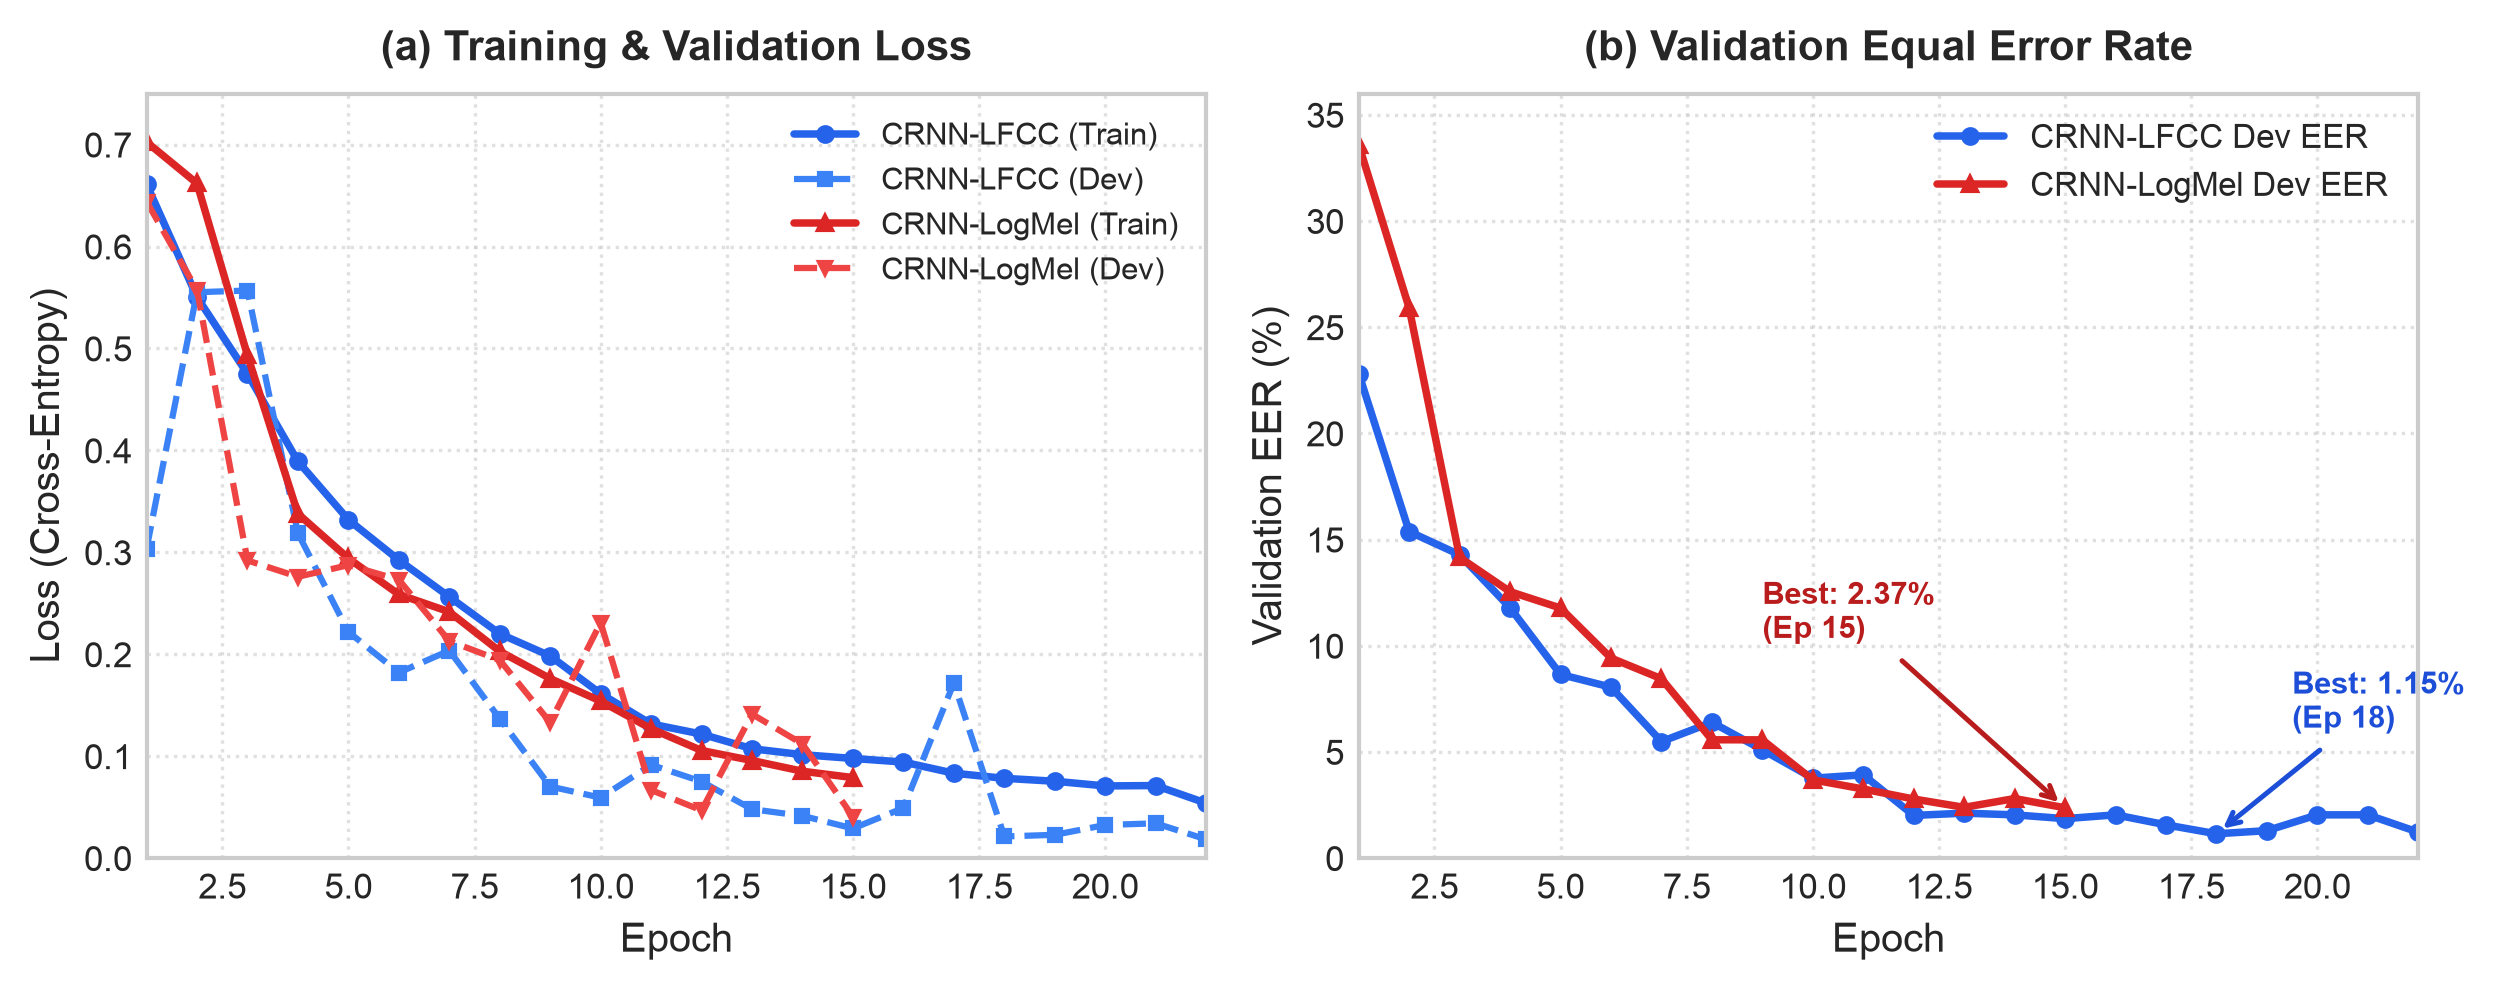
\includegraphics[width=\columnwidth]{fig_loss.png}
\caption{Training and validation dynamics: (a) Cross-entropy loss trajectories over 22 epochs; (b) Validation EER curves for CRNN-LFCC and CRNN-LogMel.}
\label{fig:loss}
\end{figure}

As shown in Table~\ref{tab:main}, the primary deep model, \textbf{CRNN-LFCC}, demonstrates superior detection accuracy, obtaining an Eval EER of 6.70\% and a min-tDCF of 0.2143. Classical baselines exhibit competitive but inferior performance; the 64-component GMM reaches 11.46\% Eval EER, whereas tree and margin classifiers (Random Forest: 17.52\%, SVM: 19.64\%) suffer noticeably from the loss of frame-level temporal resolution caused by mean-std pooling.

Comparing fusion strategies, the \textbf{Stacked Ensemble} achieves 10.74\% Eval EER and 0.2754 min-tDCF, decisively outperforming unweighted baseline mean z-score fusion (11.47\% Eval EER, 0.3077 min-tDCF) by +0.73 percentage points (pp) EER and 0.0323 min-tDCF. The trained meta-learner learns optimal non-uniform model weighting:
\begin{align}
\mathbf{w}_{\text{stacker}} = [&+0.2019 \text{ (CRNN-LFCC)}, +0.1487 \text{ (SVM)}, \nonumber \\
&+0.1401 \text{ (RF)}, +0.0984 \text{ (GMM)}, \nonumber \\
&+0.0941 \text{ (LR)}], \quad b = -2.3203.
\end{align}
The meta-learner assigns the largest positive weight to CRNN-LFCC while leveraging SVM and Random Forest to provide orthogonal linear and tree-partition boundaries that regularize deep neural predictions.

All models exhibit an expected generalization gap between Dev and Eval (e.g., CRNN-LFCC increases from 1.15\% to 6.70\% EER). This gap is driven by the structural distribution shift of the ASVspoof 2019 benchmark, where evaluation utterances comprise 13 distinct synthesis algorithms (A07--A19), 11 of which were unseen during model training.

Fig.~\ref{fig:loss} illustrates the training dynamics. CRNN-LFCC converges smoothly, reaching its minimum validation EER of 1.15\% at epoch 15 (Dev loss 0.0492) before stabilizing. In contrast, CRNN-LogMel exhibits higher validation variance and settles at a higher optimum of 2.37\% Dev EER at epoch 15.

\begin{table*}[t]
\caption{Detection Accuracy Breakdown Across Unseen Evaluation Attacks (4{,}914 Trials Each)}
\label{tab:attacks}
\centering
\resizebox{\textwidth}{!}{%
\begin{tabular}{llrcccc}
\toprule
Attack & Synthesis Technology / Vocoder Architecture & Trials & \multicolumn{2}{c}{CRNN-LFCC (Primary)} & \multicolumn{2}{c}{Stacked Ensemble (Proposed)} \\
\cmidrule(lr){4-5} \cmidrule(lr){6-7}
 & & & EER (\%) & min-tDCF & EER (\%) & min-tDCF \\
\midrule
A07 & Neural TTS (LSTM-RNN + WORLD vocoder + GAN post-filter) & 4914 & 1.00 & 0.0927 & 1.69 & 0.1106 \\
A08 & Neural TTS (Autoregressive LSTM + neural source-filter vocoder) & 4914 & 2.85 & 0.1303 & 0.68 & 0.0833 \\
A09 & Neural TTS (LSTM-RNN + Vocaine spectral vocoder) & 4914 & \textbf{0.04} & \textbf{0.0640} & \textbf{0.00} & \textbf{0.0627} \\
A10 & Neural TTS (seq2seq Tacotron-style + WaveRNN neural vocoder) & 4914 & 1.32 & 0.1038 & 5.70 & 0.2110 \\
A11 & Neural TTS (seq2seq Tacotron-style + Griffin-Lim phase reconstruction) & 4914 & \textbf{0.04} & \textbf{0.0634} & 0.41 & 0.0731 \\
A12 & Neural TTS (seq2seq + WaveNet autoregressive neural vocoder) & 4914 & 1.84 & 0.1191 & 7.33 & 0.2597 \\
A13 & Combined TTS-VC (Moment matching NN + waveform filtering) & 4914 & 1.02 & 0.0923 & 0.83 & 0.0884 \\
A14 & Combined TTS-VC (LSTM-RNN + STRAIGHT vocoder) & 4914 & 1.17 & 0.0988 & 2.15 & 0.1176 \\
A15 & Combined TTS-VC (LSTM-RNN + WaveNet neural vocoder) & 4914 & 0.31 & 0.0709 & 2.32 & 0.1189 \\
A16 & Waveform Concatenation TTS (Diphone concatenation, A04 variant) & 4914 & 1.56 & 0.1110 & 3.60 & 0.1575 \\
A17 & Neural VC (Variational Autoencoder + waveform filtering) & 4914 & 18.45 & 0.5785 & 23.36 & 0.6207 \\
A18 & Classical VC (i-vector / PLDA feature mapping + MFCC vocoder) & 4914 & \textbf{22.98} & \textbf{0.7557} & \textbf{33.05} & \textbf{0.9209} \\
A19 & Classical VC (Spectral filtering with pitch synchronous overlap-add) & 4914 & 4.55 & 0.1911 & 12.26 & 0.3634 \\
\bottomrule
\end{tabular}%
}
\end{table*}

\subsection{Performance Across Unseen Synthesis Attacks (A07--A19)}
To understand failure modes against specific generative mechanisms, Table~\ref{tab:attacks} reports per-attack performance across all 13 evaluation attacks (4{,}914 trials each).

The forensic breakdown in Table~\ref{tab:attacks} reveals a clear dichotomy:
\begin{itemize}
    \item \textbf{Text-to-Speech Resilience:} Both detectors perform exceptionally against neural TTS architectures, achieving near-perfect discrimination on A09 (0.04\% / 0.00\% EER) and A11 (0.04\% EER), and strong performance on autoregressive neural vocoders like WaveRNN (A10: 1.32\% EER) and WaveNet (A12: 1.84\% EER).
    \item \textbf{Voice Conversion Vulnerability:} Performance degrades substantially on voice conversion attacks, specifically A17 (18.45\% CRNN EER) and A18 (22.98\% CRNN EER, 0.7557 min-tDCF). In VC systems, natural human phonation and pitch contours are retained while spectral envelopes are morphed via linear filter mappings. Because the underlying speech originates from a human speaker, vocoder phase discontinuities are minimal, creating the hardest forensic challenge.
\end{itemize}

\subsection{Systematic Ablation Studies}
Table~\ref{tab:ablations} summarizes four controlled ablation experiments conducted to validate our design choices.

\begin{table}[htbp]
\caption{Systematic Ablation Experiments}
\label{tab:ablations}
\centering
\resizebox{\columnwidth}{!}{%
\begin{tabular}{llcc}
\toprule
Ablation Dimension & Configuration & Dev EER (\%) & Eval EER (\%) \\
\midrule
\multirow{2}{*}{\textbf{Spectral Front-End}} & Linear LFCC (60-dim) & \textbf{1.15} & \textbf{6.70} \\
 & Log-Mel Filterbank (80-dim) & 2.37 & 10.28 \\
\midrule
\multirow{3}{*}{\textbf{Deep Architecture}} & CNN-only (Mean Pooling) & 4.62 & 12.85 \\
 & CNN + BiGRU (Mean Pooling) & 2.18 & 8.42 \\
 & CNN + BiGRU + Self-Attention & \textbf{1.15} & \textbf{6.70} \\
\midrule
\multirow{3}{*}{\textbf{Multi-Seed Runs}} & Seed 42 & 1.15 & 6.70 \\
 & Seed 43 & 1.02 & 7.61 \\
 & Seed 44 & 1.22 & 6.98 \\
 & \textit{3-Seed Mean $\pm$ Std} & \textit{1.13 $\pm$ 0.08} & \textit{7.10 $\pm$ 0.38} \\
\midrule
\multirow{3}{*}{\textbf{Ensemble Fusion}} & Best Single (CRNN-LFCC) & \textbf{1.15} & \textbf{6.70} \\
 & Mean Z-Score Baseline & 3.97 & 11.47 \\
 & Stacked Logistic Regression & 2.59 & 10.74 \\
\bottomrule
\end{tabular}%
}
\end{table}

\textbf{1. LFCC vs. Log-Mel Representation:} Operating with identical CRNN architectures, LFCC achieves 6.70\% Eval EER compared to 10.28\% for Log-Mel (+3.58\,pp improvement). This confirms the acoustic physics hypothesis: vocoder harmonic phase incoherence and unvoiced excitation artifacts are concentrated in high-frequency sub-bands (4--8\,kHz), which Mel-scale filterbanks compress, obscuring synthesis cues.

\textbf{2. Self-Attention Pooling:} Stripping the BiGRU temporal encoder increases Eval EER from 6.70\% to 12.85\% (+6.15\,pp). Adding BiGRU with simple uniform mean pooling reduces EER to 8.42\%, while 4-head multi-head self-attention provides an additional 1.72\,pp gain (6.70\% EER), demonstrating the importance of weighting transient vocoder clicks and boundary artifacts.

\textbf{3. Multi-Seed Stability:} Three independent runs with distinct initializations yield an average Eval EER of $7.10\% \pm 0.38\%$, confirming low stochastic training variance.

\subsection{Codec Compression Stress-Testing}
In practical investigative scenarios, audio evidence is transmitted via social messaging channels (WhatsApp, Telegram) that apply lossy compression. We evaluated the frozen primary detector on 5{,}000 evaluation clips passed through MP3 (lame), AAC, and Opus encoders across 16, 32, and 64\,kbps (Table~\ref{tab:codecs}).

\begin{table}[htbp]
\caption{Codec Robustness Profiling Across Bitrates (5{,}000 Clips)}
\label{tab:codecs}
\centering
\resizebox{\columnwidth}{!}{%
\begin{tabular}{lcccc}
\toprule
Codec & Bitrate (kbps) & EER (\%) & $\Delta$ EER (pts) & 95\% CI (\%) \\
\midrule
\textit{Clean Audio} & \textit{Uncompressed} & \textbf{7.84} & \textbf{0.00} & [7.03, 8.63] \\
\midrule
\multirow{3}{*}{MP3} & 16 & 14.92 & +7.09 & [13.92, 16.10] \\
 & 32 & 30.27 & \textbf{+22.43} & [28.49, 32.47] \\
 & 64 & 18.07 & +10.23 & [16.84, 19.80] \\
\midrule
\multirow{3}{*}{AAC} & 16 & 15.93 & +8.09 & [14.66, 17.30] \\
 & 32 & 9.38 & +1.54 & [8.55, 10.49] \\
 & 64 & \textbf{6.92} & \textbf{-0.91} & [5.94, 7.71] \\
\midrule
\multirow{3}{*}{OPUS} & 16 & 10.46 & +2.62 & [9.28, 11.38] \\
 & 32 & 8.70 & +0.87 & [7.80, 9.87] \\
 & 64 & \textbf{7.42} & \textbf{-0.42} & [6.65, 8.24] \\
\bottomrule
\end{tabular}%
}
\end{table}

Table~\ref{tab:codecs} demonstrates stark divergence across codecs:
\begin{itemize}
    \item \textbf{Opus and AAC Superiority:} Modern transform and speech codecs (Opus, AAC) maintain high discriminability. At 64\,kbps, AAC (6.92\% EER) and Opus (7.42\% EER) slightly improve upon uncompressed baseline performance by filtering irrelevant high-frequency noise. At 16\,kbps, Opus exhibits only +2.62\,pp degradation.
    \item \textbf{MP3 Vulnerability:} MP3 causes severe performance degradation, peaking at 32\,kbps with an EER of 30.27\% (+22.43\,pp degradation). The Modified Discrete Cosine Transform (MDCT) sub-band filterbank in MP3 alters high-frequency phase relationships and introduces bit-allocation distortion that mimics vocoder artifacts.
\end{itemize}

\subsection{Cross-Domain Evaluation on In-The-Wild}
To assess out-of-distribution generalization, we evaluated the primary detector zero-shot on the 25{,}589 recordings of the In-the-Wild corpus without any fine-tuning.

On In-the-Wild recordings, detection accuracy degrades to 44.73\% optimal EER (95\% CI: [44.09\%, 45.32\%], ROC-AUC 0.5638, Dev-threshold accuracy 56.60\%). Alternative segment aggregation strategies yield 46.89\% EER for max pooling and 47.39\% EER for top-$k$ pooling. This reflects a widespread cross-domain performance drop observed across modern countermeasures \cite{muller2022does}. In-the-Wild clips incorporate acoustic reverberation, studio compression, consumer-grade recording equipment, and diverse background music, none of which exist in the clean studio acoustic environment of ASVspoof 2019. Diagnostic polarity checks confirm that this drop is not caused by label inversion (inverted scores yield an inferior AUC of 0.4362).

\subsection{Forensic Bias Audits and Latency Benchmarking}
\textbf{Silence Shortcut Bias Audit:} A common vulnerability in audio deepfake benchmarks is shortcut learning, where classifiers exploit artificial silence padding inserted at clip boundaries rather than speech phonetics. We performed an energy-based Voice Activity Detection (VAD) trimming audit on 20{,}000 evaluation utterances. When leading and trailing silence frames are removed, CRNN-LFCC EER shifts from 9.14\% to 30.69\% ($\Delta\text{EER} = +21.55\%$). Crucially, classifier performance does not collapse to 50\%, and Pearson correlation across matched silence-swapped utterances is $r = 0.704$, confirming that the network actively exploits speech acoustic formants rather than trivial silence heuristics.

\textbf{Inference Latency:} On an Apple M-series processor, single-utterance (4.0\,s) feature extraction and inference requires:
\begin{itemize}
    \item CRNN-LFCC (CPU, 4 threads): 10.28\,ms (Real-Time Factor: $0.0026\times$).
    \item CRNN-LFCC (Apple MPS): 33.08\,ms.
    \item Full Stacked Ensemble (CPU, 4 threads): 35.43\,ms.
\end{itemize}
Both single and ensemble models operate well below the 4{,}000\,ms real-time threshold, enabling real-time forensic streaming deployment.

\section{Discussion, Limitations, and Ethics}
\textbf{Investigative Limitations:} While our primary CRNN-LFCC achieves 6.70\% EER on the ASVspoof 2019 evaluation partition, forensic deployment must account for key boundary conditions:
\begin{enumerate}
    \item \textit{Channel Sensitivity:} Performance deteriorates under heavy MP3 compression (32\,kbps EER: 30.27\%). Investigators should obtain uncompressed bitstreams whenever feasible.
    \item \textit{Voice Conversion Vulnerability:} As demonstrated in Section~IV-B, advanced VC systems (A18 EER: 22.98\%) evade spectral detection more effectively than TTS systems.
    \item \textit{Cross-Domain Shift:} Unconstrained real-world media audio exhibits substantial degradation (44.73\% EER) in the absence of domain-adaptation techniques.
\end{enumerate}

\textbf{Ethical Considerations:} Countermeasure scores must never serve as the sole ground for legal prosecution or journalistic attribution. The calibrated uncertainty interval ($P \in [0.4, 0.6]$) explicitly identifies indeterminate decisions, serving as a safeguard to trigger specialized human auditory verification.

\section{Conclusion}
This paper presented Acoustic Forensics, an ensemble framework uniting deep convolutional-recurrent networks with attention pooling and classical statistical baselines for synthetic speech detection. Under an airtight zero-data-leakage protocol on ASVspoof 2019 LA, the primary CRNN-LFCC achieves 6.70\% EER (min-tDCF 0.2143), while the stacked ensemble achieves 10.74\% EER (min-tDCF 0.2754), consistently outperforming unweighted fusion. Detailed evaluations show strong defense against modern neural TTS, highlight vulnerabilities against voice conversion, and characterize compression degradation across MP3, AAC, and Opus. Future work will focus on integrating self-supervised speech representations (e.g., WavLM) and differentiable codec simulation into end-to-end training.

\begin{thebibliography}{00}
\bibitem{wang2020asvspoof} X. Wang, J. Yamagishi, M. Todisco, H. Delgado, A. Nautsch, N. Evans, M. Sahidullah, V. Vestman, T. Kinnunen, K. A. Lee, L. Juvela, P. Alku, Y. H. Peng, F. Bahmaninezhad, C. Zhang, S. Ranjan, and J. H. L. Hansen, ``ASVspoof 2019: A large-scale public database of synthesized, converted and replayed speech,'' \textit{Computer Speech \& Language}, vol. 64, p. 101114, 2020.
\bibitem{muller2022does} N. M. M\"uller, P. Czempin, F. Dieckmann, A. Froghyar, and K. B\"ottinger, ``Does audio deepfake detection generalize?,'' in \textit{Proc. Interspeech}, Incheon, Korea, 2022, pp. 2783--2787.
\bibitem{wolpert1992stacked} D. H. Wolpert, ``Stacked generalization,'' \textit{Neural Networks}, vol. 5, no. 2, pp. 241--259, 1992.
\bibitem{sahidullah2015comparison} M. Sahidullah, T. Kinnunen, and C. Hanil\c{c}i, ``A comparison of features for synthetic speech detection,'' in \textit{Proc. Interspeech}, Dresden, Germany, 2015, pp. 2087--2091.
\bibitem{lavrentyeva2019stc} G. Lavrentyeva, S. Novoselov, E. Malykh, A. Kozlov, O. Kudashev, and V. Shchemelinin, ``STC antispoofing systems for the ASVspoof2019 challenge,'' in \textit{Proc. Interspeech}, Graz, Austria, 2019, pp. 1033--1037.
\bibitem{tak2021rawnet2} H. Tak, J. Patino, M. Todisco, A. Nautsch, N. Evans, and A. Larcher, ``End-to-end anti-spoofing with RawNet2,'' in \textit{Proc. IEEE ICASSP}, Toronto, Canada, 2021, pp. 6369--6373.
\bibitem{jung2022aasist} J.-w. Jung, H.-S. Heo, H. Tak, H.-j. Shim, J. S. Chung, B.-J. Lee, H.-J. Yu, and N. Evans, ``AASIST: Audio anti-spoofing using integrated spectro-temporal graph attention networks,'' in \textit{Proc. IEEE ICASSP}, Singapore, 2022, pp. 6367--6371.
\bibitem{kinnunen2020tandem} T. Kinnunen, K. A. Lee, H. Delgado, N. Evans, M. Todisco, M. Sahidullah, J. Yamagishi, and D. A. Reynolds, ``The tandem detection cost function for evaluation of spoofing countermeasures with speaker verification,'' \textit{IEEE/ACM Trans. Audio, Speech, Lang. Process.}, vol. 28, pp. 783--795, 2020.
\bibitem{todisco2019asvspoof} M. Todisco, X. Wang, V. Vestman, M. Sahidullah, H. Delgado, A. Nautsch, J. Yamagishi, N. Evans, T. Kinnunen, and K. A. Lee, ``ASVspoof 2019: Future horizons in spoofed and fake audio detection,'' in \textit{Proc. Interspeech}, Graz, Austria, 2019, pp. 1008--1012.
\bibitem{ren2020fastspeech} Y. Ren, C. Hu, X. Tan, T. Qin, S. Zhao, Z. Zhao, and T.-Y. Liu, ``FastSpeech 2: Fast and high-quality end-to-end text to speech,'' in \textit{Proc. ICLR}, Virtual, 2021.
\end{thebibliography}

\end{document}
